\documentclass[conference]{IEEEtran}

\usepackage[pdftex]{graphicx}
\usepackage{graphicx}
\usepackage[backend=biber,bibstyle=numeric,sorting=ynt]{biblatex}
\addbibresource{references.bib}
\usepackage[colorlinks=true, allcolors=blue]{hyperref}

\usepackage{fancyhdr}
\pagestyle{fancy}
\fancyhf{}
\cfoot{\thepage}

\begin{document}

\title{Mammographic Mass Data Set}

\author{\IEEEauthorblockN{Pedro Sobral - 98491  - (50\%) - sobral@ua.pt,
Eva Bartolomeu - 98513 - (50\%) - evabartolomeu@ua.pt}
\IEEEauthorblockA{Departamento de Eletrónica, Telecomunicações e Informática,
University of Aveiro, Portugal\\
Fundamentos de Aprendizagem Automática
 - Course Instructor: Pétia Georgieva}}
\maketitle

\maketitle

% As a general rule, do not put math, special symbols or citations
% in the abstract or keywords.
\begin{abstract}
The main goal of this project is to apply suitable machine learning algorithms learned in class to solve a specific data science problem, in this case, models capable of identifying benign or malignant masses in mammography's. In this report, we try to obtain the best result of the accuracy of the implemented models.
\end{abstract}

\begin{IEEEkeywords}
Machine Learning, Classification Model, Logistic Regression, SVM, Neural Network, Normalization
\end{IEEEkeywords}

\IEEEpeerreviewmaketitle

\section{Introduction}
In the scope of the subject Fundamentals of Automatic Learning, a work was proposed on a problem (of our choice) of machine learning. The goal of this project is to apply suitable machine learning algorithms learned in class or self-learned to solve a specific data science problem (classification, regression, clustering). Represent the results in graphical/table formats and make analysis and conclusions.
We decided to choose project proposal 3, Mammographic Mass Data Set. This data set can be used to predict the severity (benign or malignant) of a mammographic mass lesion from BI-RADS attributes and the patient's age. The aim is to discriminate benign from malignant cases assuming that all cases with BI-RADS assessments greater or equal a given value (varying from 1 to 5), are malignant and the other cases are benign. We chose this theme because we already work on project with a similar theme.

\section{Data Description and Preprocessing}
\subsection{Data Description}

Mammography is the most effective method for breast cancer \cite{mammographymosteffectivemethod} \cite{mammographybestmethod} screening available today. However, the low positive predictive value of breast biopsy resulting from mammogram interpretation leads to approximately 70\% unnecessary biopsies with benign outcomes. 

To reduce the high number of unnecessary breast biopsies, several computer-aided diagnosis (CAD) systems have been proposed in the last few years. This data set \cite{dataset} can be used to predict the severity (benign or malignant) of a mammographic mass lesion from BI-RADS attributes and the patient's age.

It contains a BI-RADS assessment, the patient's age, and three BI-RADS attributes (Shape, Margin, Density) together with the ground truth (the severity field) for 516 benign and 445 malignant masses that have been identified on full-field digital mammograms collected at the Institute of Radiology of the University Erlangen-Nuremberg between 2003 and 2006. Each instance has an associated BI-RADS assessment ranging from 1 (definitely benign) to 5 (highly suggestive of malignancy).\\
The attributes of the data-set are the following:
\begin{itemize}
  \item BI-RADS assessment: 1 to 5 (ordinal)  
  \item Age: patient's age in years (integer)
  \item Shape: mass shape: round=1 oval=2 lobular=3 irregular=4 (nominal)
  \item Density: mass density high=1 iso=2 low=3 fat-containing=4 (ordinal)
  \item Severity: benign=0 or malignant=1 (binominal)
\end{itemize}

\subsection{Data Preprocessing}

First of all, we notice that the original data-set has missing values, so on loading the data we substituted all the missing values with NaN, after that, we replaced those values with the mean of the particular attribute. The data-set contains some outliers in the BI-RADS attribute, in order to solve that we removed all the lines with outliers.

We decided to apply a normalization approach. Normalization is a re-scaling technique, that re-scaling an input variable to the range between 0 and 1.

\section{Data Visualization}

In order to have deep knowledge about the data-set it is important to have many data visualization plots such as Box, Histograms, and Scatter. These plots help to understand more how the data are correlated.
The data-set is balanced, this is important so that we have more chance that the model will be certain because the data is well distributed and non-bias. The next figure (Fig. \ref{img:severity_distribution}) shows that the number of Benign and Malign cases is very identical.

\begin{figure}[!h]
    \centering
    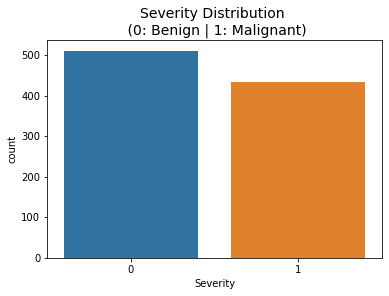
\includegraphics[width=3.0in]{severity_distribution.png}
    \caption{Class Distribution}
    \label{img:severity_distribution}
\end{figure}

The percentages of the Severity are the following (Fig. \ref{img:perc_dist.png}).
\begin{figure}[!h]
    \centering
    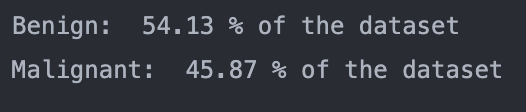
\includegraphics[width=3.0in]{perc_dist.png}
    \caption{Percentages of the Severity Distribution}
    \label{img:perc_dist.png}
\end{figure}

In order to can see some pattern in the data, we plot all the data, like the following figure \ref{img:data.png} shows.

\begin{figure}[!h]
    \centering
    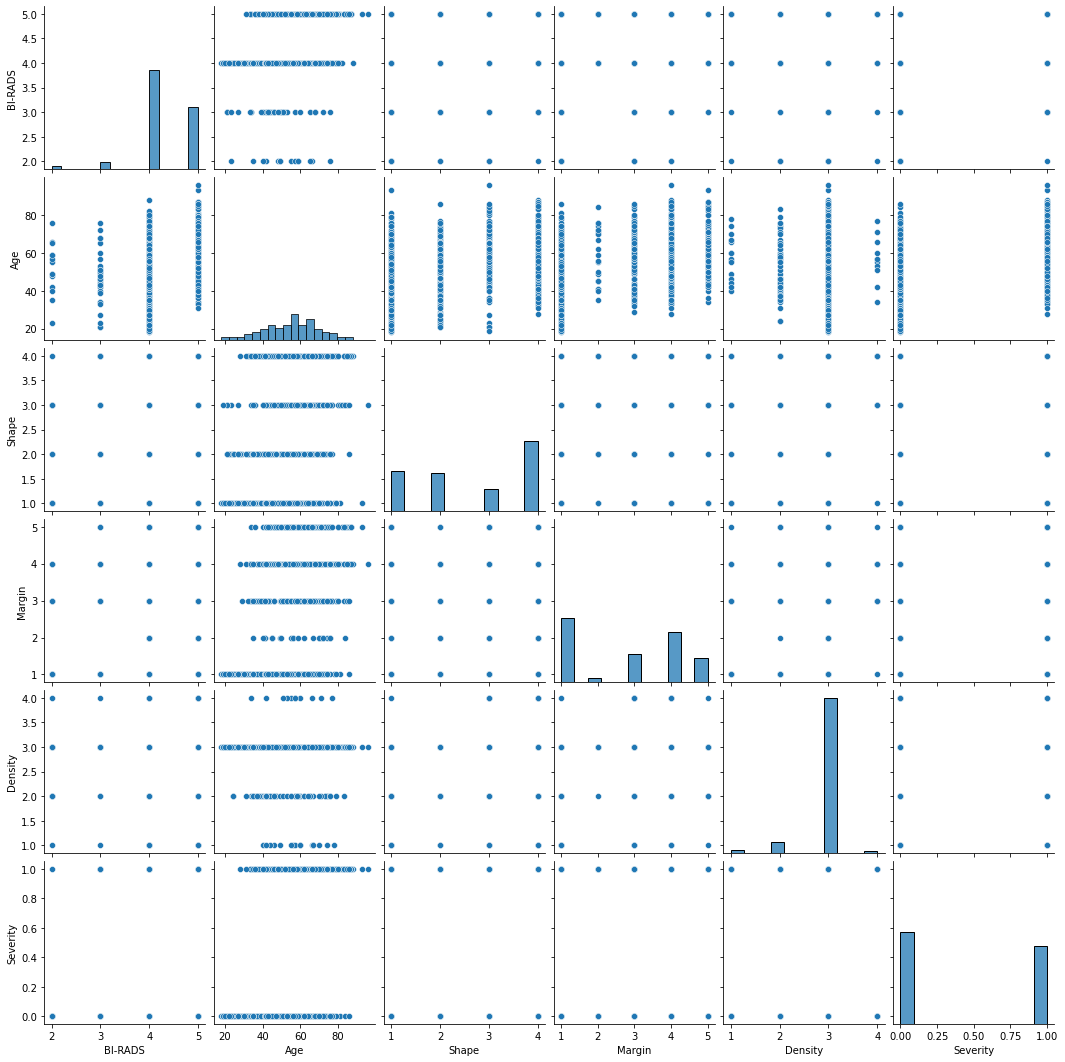
\includegraphics[width=3.0in]{data.png}
    \caption{Data}
    \label{img:data.png}
\end{figure}

To see the attribute distributions we make some histograms, ones with benign (Fig. \ref{img:hist_benign.png}) cases and others with malignant (Fig. \ref{img:hist_malignant.png}) cases.
We make as well a Boxplot graphic to show all the features with the \textbf{Severity} (Fig \ref{img:box_plot.png}).

\begin{figure}[!h]
    \centering
    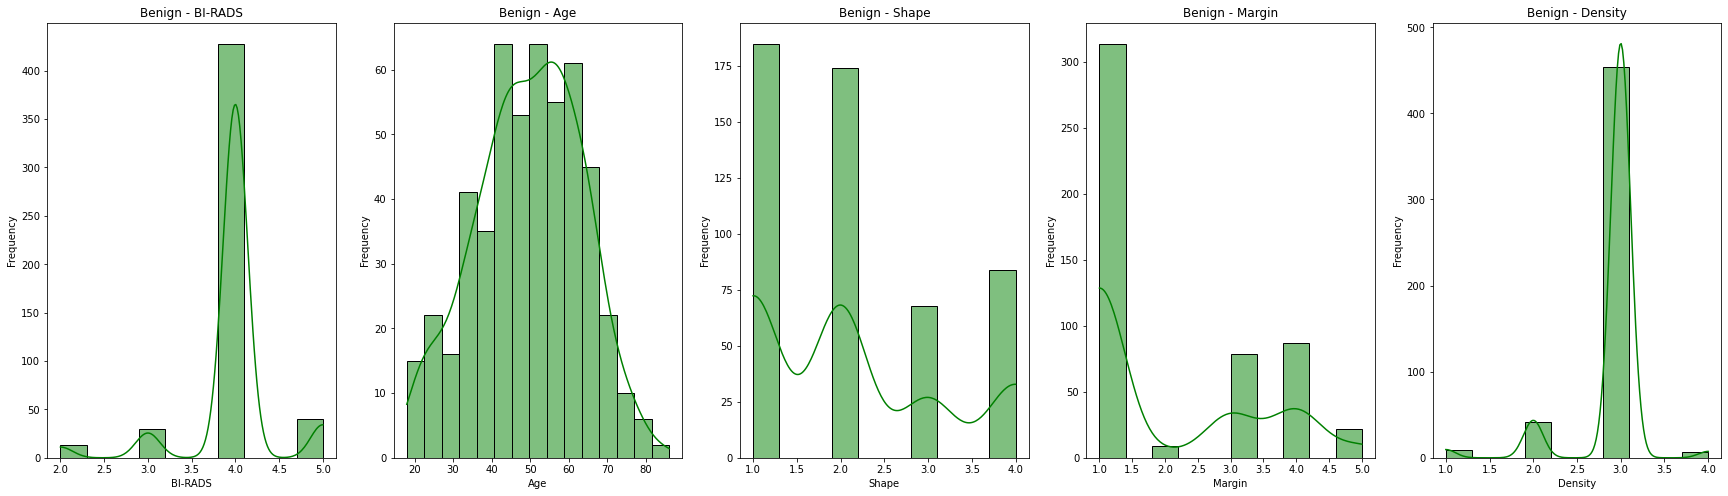
\includegraphics[width=3.0in]{hist_benign.png}
    \caption{Histograms - Benign}
    \label{img:hist_benign.png}
\end{figure}

\begin{figure}[!h]
    \centering
    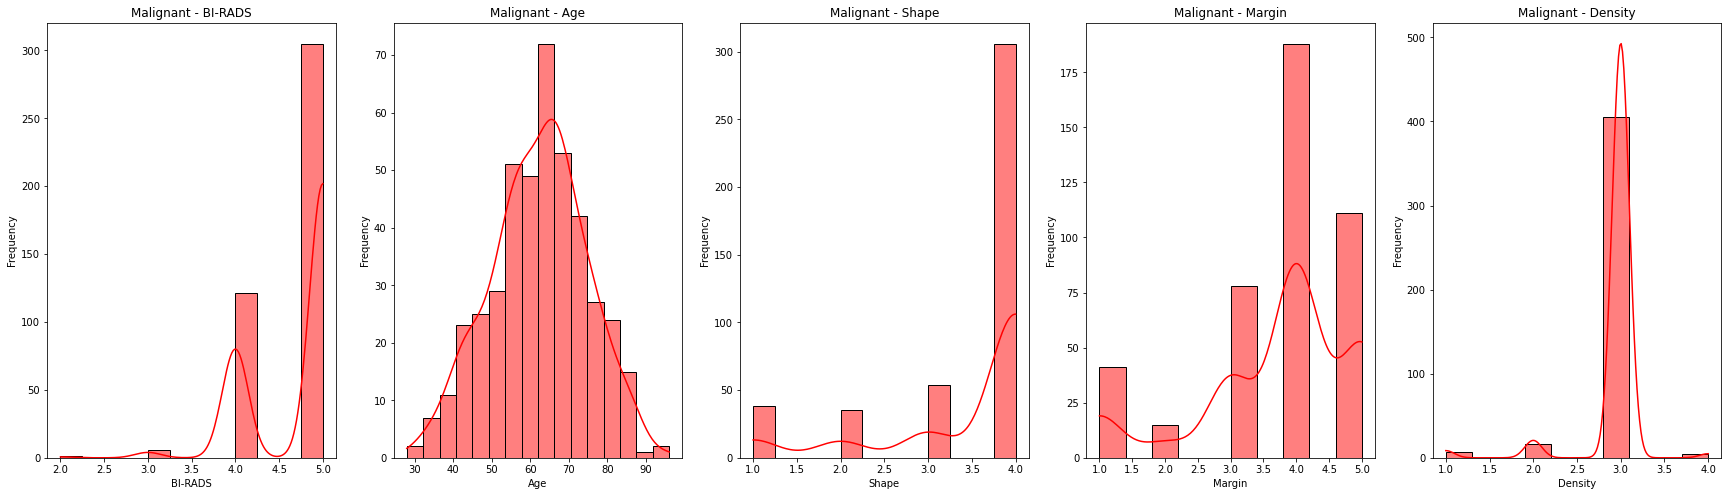
\includegraphics[width=3.0in]{hist_malignant.png}
    \caption{Histograms - Malignant}
    \label{img:hist_malignant.png}
\end{figure}

Here we can see that the malignant cases, for example, are often in ages from 50 to 80, however, the benign cases appear earlier and with a bigger frequency, but in a general analysis the histograms are identical. A very obvious consideration to make is that it is more probable to have a malignant case if the attribute "\textbf{Shape}" is 4. About "\textbf{Margin} " level, how higher the value of the attribute more malignant cases are, make the comparison with the "\textbf{Margin}" in the benign histograms, where tendentiously the benign cases have a lower value to this attribute. About "\textbf{Density}" there are no assumptions to make since the histograms are very similar, as is possible to observe in the figures.

\begin{figure}[!h]
    \centering
    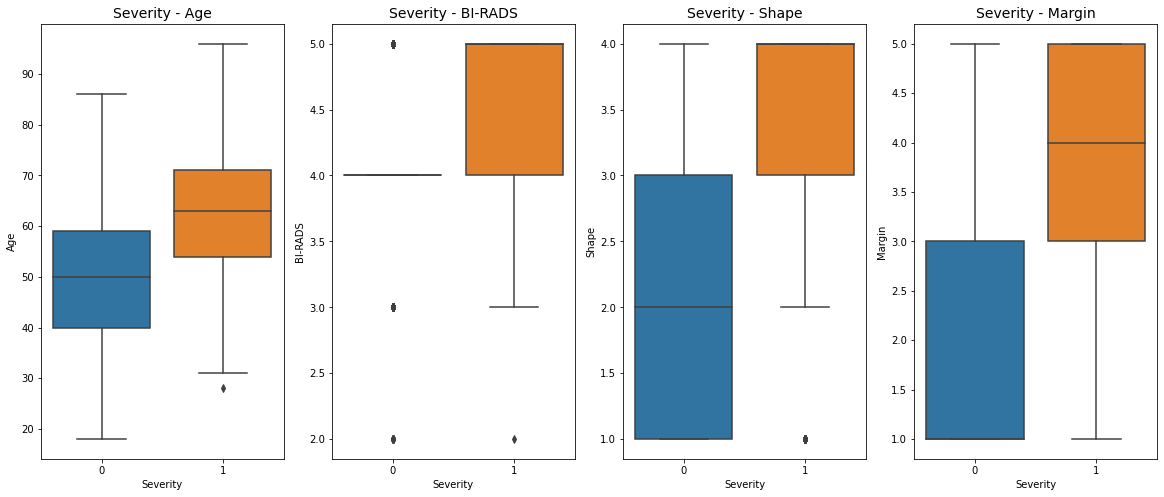
\includegraphics[width=3.0in]{box_plot.png}
    \caption{Feature BoxPlot}
    \label{img:box_plot.png}
\end{figure}



So, in order to clarify this situation, and identify the most contributed features to our prediction model it is a good way to improve the accuracy of the data-set, eliminating the least contributed features. 

A good first way to make some assumptions is by plotting a Correlation Matrix (Fig. \ref{img:corr_matrix}), this matrix is good to verify the coefficients of connection between the features. Analyzing the matrix, the less contributed feature is the "\textbf{Density}", this attribute has the lowest values in the correlation matrix, as it is possible to see, it has a white color, so it means it is very low.

\begin{figure}[!h]
    \centering
    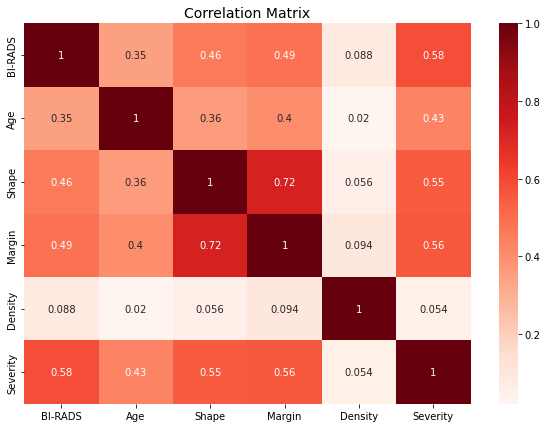
\includegraphics[width=3.0in]{corr_matrix.png}
    \caption{Correlation Matrix}
    \label{img:corr_matrix}
\end{figure}

We have done some research \cite{featureelimination} and decide to implement two techniques, the RFE and the PCA.

The RFE technique \cite{rfe} is an algorithm that returns the feature's importance from the current set of features. So was implemented this algorithm to return the 3 most important features. The output of this implementation is demonstrated in Fig \ref{img:rfe.png}. 

\begin{figure}[!h]
    \centering
    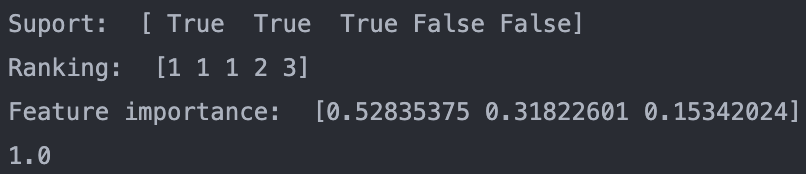
\includegraphics[width=3.0in]{rfe.png}
    \caption{RFE}
    \label{img:rfe.png}
\end{figure}

With these results, the most important features are the first three: \textbf{BI-RADS}, \textbf{Age}, and \textbf{Margin}. Being the least important the \textbf{Margin} and \textbf{Density}.

Using the PCA technique \cite{pca},  is the main linear algorithm for dimension reduction, this algorithm identifies and discards features that are less useful to make a valid approximation on a data-set.
With this, we obtain the following results (0.478 + 0.204 + 0.143) with a sum of (~83\%) for the 3 most important features. (Fig. \ref{img:pca.png})

\begin{figure}[!h]
    \centering
    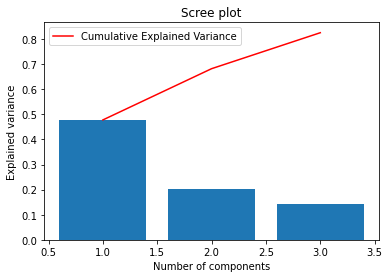
\includegraphics[width=3.0in]{pca.png}
    \caption{PCA}
    \label{img:pca.png}
\end{figure}

So with all this information, we decided to remove the \textbf{Margin} and \textbf{Density} features of our data-set, remaining with the features \textbf{BI-RADS}, \textbf{Age} and \textbf{Margin}.

\section{Machine Learning Models}

Before implementing the machine learning models, we decided that 25\% of the data will be used for testing and 75\% of the data will be used for training. For this we created two sets, the test, and the training, using the sklearn.model\_ selection.train\_ test\_ split library \cite{train-test-split}.

In each implemented machine learning algorithm, we run the algorithm with the base model, with the hyper-parameter selection model, and with K-Fold Cross Validation on the hyper-parameter selection model. For the execution of the described models, we created a function that trains the model passed as an argument and shows graphs, tables, and data in the output, in order to facilitate the analysis of the model.
We also implemented a function that, through the sklearn.model\_selection. GridSearchCV library \cite{grid-search-cV}, performs an exhaustive search on a list of parameters, training a given model with all the parameters, in the end, we return the parameters that gave the best performance, according to the accuracy strategy.

We developed a function that splits the data set into k mixed sets, with training/test indices, using the sklearn.model\_selection.KFold feature \cite{k-fold}. Still, within the function, we evaluate the metrics by cross-validation and record the fit/score times through sklearn.model\_selection.cross\_validate \cite{cross-validate}.

Finally, we create a function that calculates training and testing scores for an estimator with several different values on a specific parameter, these calculations are performed with the sklearn.model\_selection.validation\_curve \cite{validation-curve}. We then graphed the average training scores, and the average test scores, on each specific parameter value.

\subsection{Logistic Regression}
The Logistic Regression \cite{logistic-regression-def} algorithm determines the probability of a binary event (which has only two different results). The Logistic Regression category is supervised learning.

In our problem, we use this algorithm, where the binary results are malignant or benign cancer. We performed the algorithm using the sklearn.linear\_model.LogisticRegression library \cite{logistic-regression}, and with the previously described functions.

\subsection{Neural Network}
Neural Network \cite{neural-networks-def} is a deep learning algorithm, which teaches you to process data like a human brain. It uses interconnected nodes much like neurons, and teaches computers to learn from mistakes and improve. We implemented this algorithm with the sklearn.neural\_network.MLPClassifier library \cite{MLPClassifier}.

\subsection{Support Vector Machine}
SVM \cite{svm-def} is a supervised learning algorithm, which analyzes data for classification and regression observation. Considering a set of training examples, where each example belongs to a category (there are two categories, two results), the SVM algorithm builds a model that classifies new data to a category. This classifier is a non-probabilistic linear binary. Examples are mapped to points in space, with a wide gap between categories. We use sklearn.svm.SVC \cite{svm} to develop this algorithm.

\subsection{k-Nearest Neighbor}
k-NN \cite{knn-def} is a non-parametric, supervised learning algorithm that uses the proximity of points to classify or predict, assuming that similar points are close. We implemented the algorithm using the sklearn.neighbors.KNeighborsClassifier \cite{knn} library.

\subsection{Decision Tree}
Decision Tree \cite{tree-def} is supervised learning, presents a tree structure, the internal nodes are the characteristics of a dataset, the branches are the decision conditions, and the leaf nodes are the results. Graphically represents all possible solutions to a problem. In the development of the algorithm, we used sklearn.tree\_DecisionTreeClassifier \cite{tree}.

\section{Results}

\subsection{Logistic Regression}

First, we run this algorithm with the base model, with the hyper-parameter selection model, and with K-Fold cross-validation on the hyper-parameter selection model. In Table \ref{tab:tab1} we can see the parameters chosen in the hyper-parameter selection model.

\begin{table}[ht]
    \centering
    \caption{Best parameters in Logistic Regression} 
    \begin{tabular}{||c c c c c||} 
     \hline
     C & class\_weight & max\_iter & penalty & solver \\ [0.5ex] 
     \hline\hline
     10 & balanced & 100 & l2 & liblinear \\ 
    \hline
    \end{tabular}
    \label{tab:tab1}
\end{table}

The value selected for parameter C was 10. The higher the value of this parameter, the greater the weight on the training data and the lower the weight on the complexity penalty. The smaller the value of this parameter, the smaller the weight in the training data and the greater the weight in the complexity penalty. This parameter is used to handle extreme data. 

The parameter selected in the class\_weight was “balanced”, this strategy implicitly replicates the class with the lowest weight, until there is the same number of samples as the class with the highest weight.

The chosen max\_iter was 100, that is, the maximum number of iterations for the solvers to converge is 100.

The “l2” parameter was selected for the penalty. This parameter imposes the penalty of the square of the magnitude of the coefficients in the model. Thus reducing the coefficients with less contribution, that is, regularization is performed.

The parameter chosen in the solver was “liblinear”, this strategy is advised in small data sets, such as our set. This strategy behaves like a multiclass classified, through the coordinate descent algorithm, ie, separate binary classifiers are trained for all classes.

\subsubsection{Base Model}
The results for the Base Model application are:

\begin{figure}[!h!]
    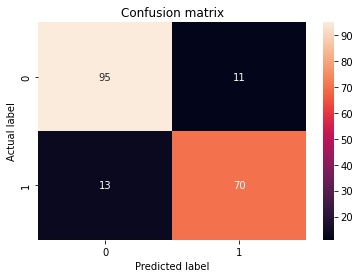
\includegraphics[width=4.5cm]{LogReg/lg1_1.png}%
    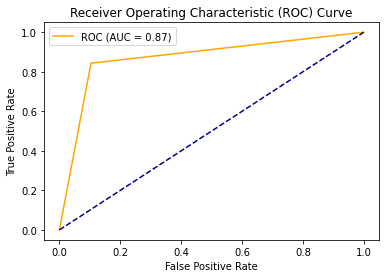
\includegraphics[width=4.5cm]{LogReg/lg1_2.png}%
    \caption{Confusion Matrix & ROC Curve}%
    \label{fig:conf_LogReg_1}%
\end{figure}

\subsubsection{Hyper-Parameter Selection Model}

The results for the Hyper-Parameter Selection Model are:

\begin{figure}[!h!]
    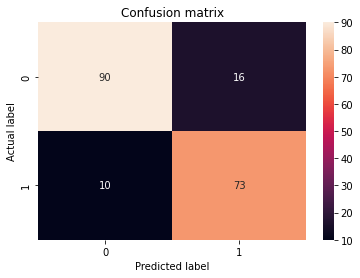
\includegraphics[width=4.5cm]{LogReg/lg2_1.png}%
    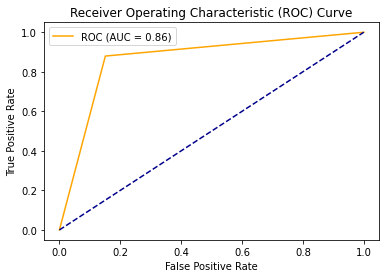
\includegraphics[width=4.5cm]{LogReg/lg2_2.png}%
    \caption{2 Confusion Matrix & ROC Curve}%
    \label{fig:conf_LogReg_2}%
\end{figure}

\subsubsection{K-Fold Cross-Validation Model}

The results for the K-Fold Cross-Validation Model are:

\begin{figure}[!h!]
    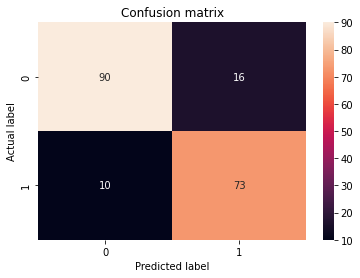
\includegraphics[width=4.5cm]{LogReg/lg3_1.png}%
    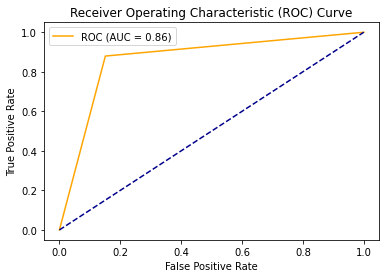
\includegraphics[width=4.5cm]{LogReg/lg3_2.png}%
    \caption{Confusion Matrix & ROC Curve}%
    \label{fig:conf_LogReg_3}%
\end{figure}

\begin{figure}[!h!]
    \centering
    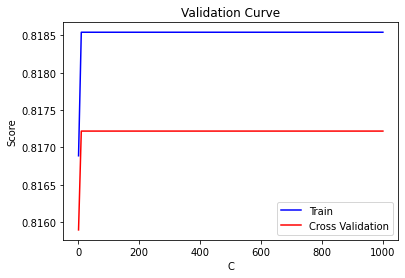
\includegraphics[width=5cm]{LogReg/lg4.png}
    \caption{Validation Curve}
    \label{fig:validationCurveLogReg}
\end{figure}

\subsubsection{Conclusions}
Observing the confusion matrices, we can conclude that the number of incorrectly classified examples, the sum of FP and FN, (13+11=21 and 10+16=26) is very low compared to the number of correctly classified examples, sum of TP with TN (95+70 and 90+73). Therefore, we can consider the model accurate.

The higher the AUC score, the better the performance of a classifier for a given task. Therefore, through the ROC Curve graphs, we can say that the classifier performed well because the AUC value is 0.86/0.87. It has good predictive power.

In Fig \ref{fig:validationCurveLogReg}, we can conclude that any value of C would be a good parameter, although a value between 0 and 50 is best, the difference is minimal. We also observed that from a value between 0 and 50 both the accuracy of the training score and the cross-validation score remain at a value, 0.8185 and 0.8175-0.8170 respectively.

\begin{table}[ht!]
    \centering
    \caption{Classification - All Model} 
    \begin{tabular}{||c| c c c||} 
     \hline
     & Accuracy & F1 Score & True Positive Rate \\ [0.5ex] 
     \hline\hline
     Base Model &0.873 & 0.853 & 0.843 \\
     \hline
    Hyper-Parameter & 0.862 & 0.848 & 0.879 \\ 
    \hline
    K-Fold & 0.862 & 0.848 & 0.879 \\ 
    \hline
    \end{tabular}
    \label{tab:tab_LogReg}
\end{table}

By table  \ref{tab:tab_LogReg} we can verify that the Accuracy, F1 score, and True positive rate values of the 3 methods are very identical, with almost no difference in choosing the best method. The Base Model appears to have better accuracy, but the Hyper-Parameter and k-fold have a better True Positive Rate. For this problem, it is more important to have a better value of True Positive Rate than a better Accuracy, because the fewer positive cases pass as negative the better when cancer is malignant it is extremely important that it does not pass as benign.

\subsection{Neural Network}

We run this model in three different ways, the base model, the hyper-parameter selection model, and the K-Fold cross-validation with the hyper-parameter selected. The following Table \ref{tab:tab2} shows the parameters chosen by the algorithm.

\begin{table}[h!]
    \centering
    \caption{Best parameters in Neural Network} 
    \begin{tabular}{||c c c c||} 
     \hline
     activation & alpha & hidden\_layer\_sizes & learning\_rate \\[0.5ex] 
     \hline\hline
     relu & 1 & (12, 12) & constant \\ 
    \hline
    \end{tabular}
    \begin{tabular}{||c c c||}
    \hline
    learning\_rate\_init & max\_iter & solver \\ [0.5ex] 
    \hline\hline
     0.001 & 1000 & adam\\ 
    \hline
    \end{tabular}
    \label{tab:tab2}
\end{table}

\subsubsection{Base Model}
The results for the Base Model application are:

\begin{figure}[h!]
    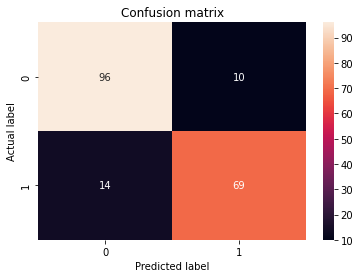
\includegraphics[width=4.5cm]{NN/nn1_1.png}%
    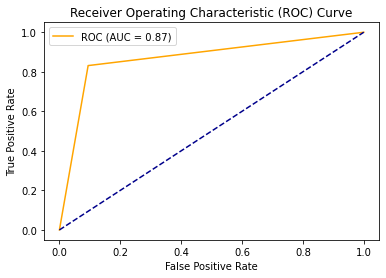
\includegraphics[width=4.5cm]{NN/nn1_2.png}%
    \caption{Confusion Matrix & ROC Curve}%
    \label{fig:conf_NN_1}%
\end{figure}

\subsubsection{Hyper-Parameter Selection Model}

The results for the Hyper-Parameter Selection Model are:

\begin{figure}[h!]
    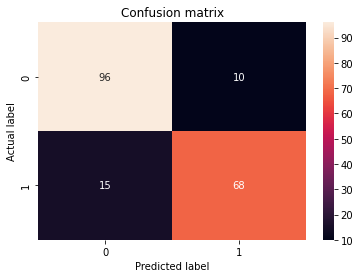
\includegraphics[width=4.5cm]{NN/nn2_1.png}%
    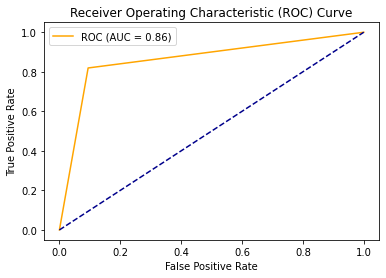
\includegraphics[width=4.5cm]{NN/nn2_2.png}%
    \caption{2 Confusion Matrix & ROC Curve}%
    \label{fig:conf_NN_2}%
\end{figure}

\subsubsection{K-Fold Cross-Validation Model}

The results for the K-Fold Cross-Validation Model are:

\begin{figure}[h!]
    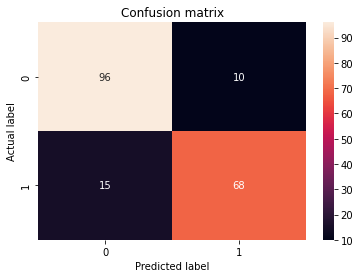
\includegraphics[width=4.5cm]{NN/nn3_1.png}%
    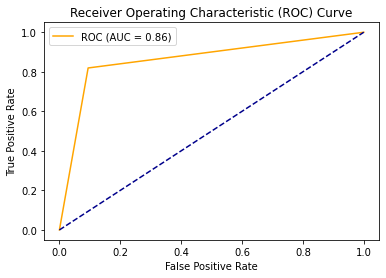
\includegraphics[width=4.5cm]{NN/nn3_2.png}%
    \caption{Confusion Matrix & ROC Curve}%
    \label{fig:conf_NN_3}%
\end{figure}

\begin{figure}[h!]
    \centering
    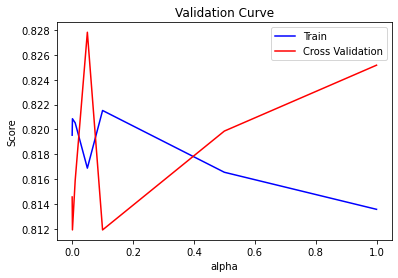
\includegraphics[width=5cm]{NN/nn3_3.png}
    \caption{Validation Curve}
    \label{img:validationCurve_NN}
\end{figure}

\subsubsection{Conclusions}
As the graphics are very identical, a general conclusion will be made about the Confusion Matrix and ROC curve of all three implementations. As we can see, Fig. \ref{fig:conf_NN_1}, \ref{fig:conf_NN_2}, \ref{fig:conf_NN_3} the Confusion Matrices are almost the same, so we see a bit of variation between the approaches, the ROC Curve is close to the top-left corner in the beginner, which is very good, how more the curve is closer to the top-left corner the better the performance, then the curve has a slope decrease to the end. About AUC (Area under the curve), how higher the value is (between 0 to 1) the better it is. As we can see in this article \cite{ROC_article}, values between 0.8 and 0.9 are considered excellent.

In Fig \ref{img:validationCurve_NN}, we can conclude that the ideal value for the alpha parameter would be 0.4 and approximately 0.01 and 0.09. We can also observe that from alpha value 0.4, the accuracy of the training score decreases, and the cross-validation score increases.

\begin{table}[ht!]
    \centering
    \caption{Classification - All Model} 
    \begin{tabular}{||c| c c c||} 
     \hline
     & Accuracy & F1 Score & True Positive Rate \\ [0.5ex] 
     \hline\hline
     Base Model &0.873 & 0.851 & 0.831 \\
     \hline
    Hyper-Parameter & 0.867 & 0.844 & 0.819 \\ 
    \hline
    K-Fold & 0.867 & 0.844 & 0.819 \\ 
    \hline
    \end{tabular}
    \label{tab:tab3}
\end{table}

So we can say \ref{tab:tab3} that with the Neural Network model, the Base Model approach is the best compared with the other two, where the \textbf{Accuracy} is 0.873 and the \textbf{True Positive Rate} is 0.831.

%%%%%%%%%%%%%%%%%%%%%%%%%%%%%%%%%%%%SVC%%%%%%%%%%%%%%%%%%%%%%%%%%%%%%%%%%%

\subsection{Support Vector Machine}

We run this model in three different ways, the base model, the hyper-parameter selection model, and the K-Fold cross-validation with the hyper-parameter selected. The following Table \ref{tab:tab-svc} shows the parameters chosen by the algorithm.

\begin{table}[h!]
    \centering
    \caption{Best parameters in SVC} 
    \begin{tabular}{||c c c c||} 
     \hline
     algorithm & n_neighbors & weights \\[0.5ex] 
     \hline\hline
     auto & 15 & uniform \\ 
    \hline
    \end{tabular}
    \label{tab:tab-svc}
\end{table}

\subsubsection{Base Model}
The results for the Base Model application are:

\begin{figure}[h!]
    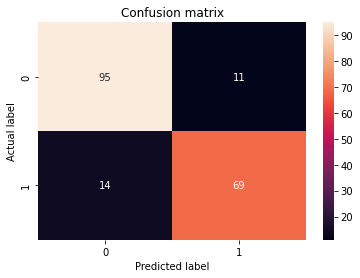
\includegraphics[width=4.5cm]{SVC/svc1_1.png}%
    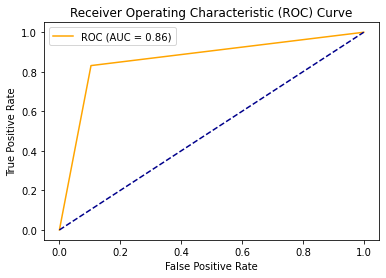
\includegraphics[width=4.5cm]{SVC/svc1_2.png}%
    \caption{Confusion Matrix & ROC Curve}%
    \label{fig:conf_SVC_1}%
\end{figure}

\subsubsection{Hyper-Parameter Selection Model}

The results for the Hyper-Parameter Selection Model are:

\begin{figure}[h!]
    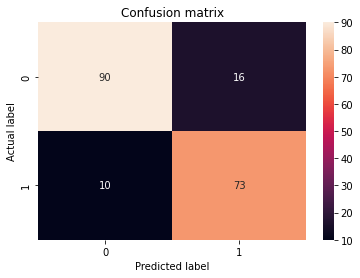
\includegraphics[width=4.5cm]{SVC/svc2_1.png}%
    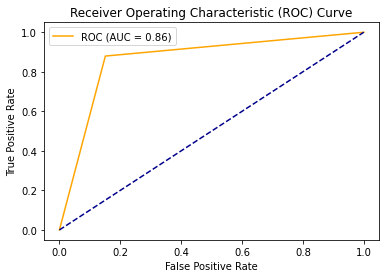
\includegraphics[width=4.5cm]{SVC/svc2_2.png}%
    \caption{2 Confusion Matrix & ROC Curve}%
    \label{fig:conf_SVC_2}%
\end{figure}

\subsubsection{K-Fold Cross-Validation Model}

The results for the K-Fold Cross-Validation Model are:

\begin{figure}[h!]
    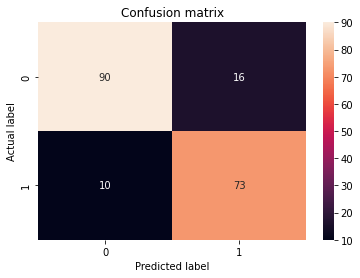
\includegraphics[width=4.5cm]{SVC/svc3_1.png}%
    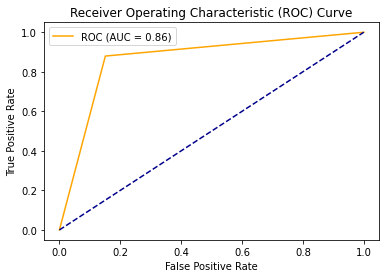
\includegraphics[width=4.5cm]{SVC/svc3_2.png}%
    \caption{Confusion Matrix & ROC Curve}%
    \label{fig:conf_SVC_3}%
\end{figure}

\begin{figure}[h!]
    \centering
    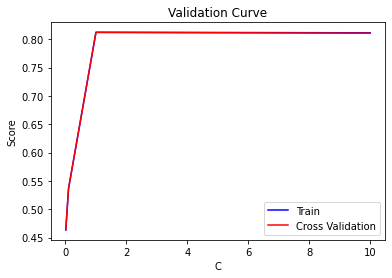
\includegraphics[width=4.5cm]{SVC/svc4_1.png}
    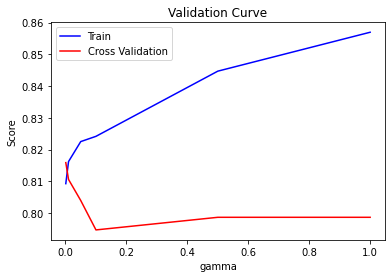
\includegraphics[width=4.5cm]{SVC/svc4_2.png}
    \caption{Validation Curve}
    \label{img:validationCurveSVC}
\end{figure}

\subsubsection{Conclusions}
As the graphics are very identical, a general conclusion will be made about the Confusion Matrix and ROC curve of all three implementations. As we can see, Fig. \ref{fig:conf_SVC_1}, \ref{fig:conf_SVC_2}, \ref{fig:conf_SVC_3} the Confusion Matrices are almost the same, so we see a bit of variation between the approaches, the ROC Curve is close to the top-left corner in the beginner, which is very good, how more the curve is closer to the top-left corner the better the performance, then the curve has a slope decrease to the end. About AUC (area under curve), how higher the value is (between 0 to 1) the better it is. As we can see in this article \cite{ROC_article}, values between 0.8 and 0.9 are considered excellent.

In Fig \ref{img:validationCurveSVC} , we can conclude that any value of C would be a good parameter, as the Train values all coincide with the Cross Validation values. We also observed that from a value of 1 of C, more and less, both the accuracy of the training score and the Cross Validation score remain at a value of 0.80.

Still in Fig \ref{img:validationCurveSVC}, we see that the ideal value for the gamma parameter is approximately 0. We also see that from a gamma value of 0, the accuracy of the training score increases, and the Cross Validation score goes down.

\begin{table}[ht!]
    \centering
    \caption{Classification - All Model} 
    \begin{tabular}{||c| c c c||} 
    \hline
     & Accuracy & F1 Score & True Positive Rate \\ [0.5ex] 
     \hline\hline
     Base Model & 0.867 & 0.846 & 0.831 \\
     \hline
    Hyper-Parameter & 0.862 & 0.848 & 0.879 \\ 
    \hline
    K-Fold & 0.862 & 0.848 & 0.879 \\ 
    \hline
    \end{tabular}
    \label{tab:tab-final-svc}
\end{table}

So we can say (Table \ref{tab:tab-final-svc}) that with the SVC model, the best approach is the Hyper-Parameter and the K-Fold, where the \textbf{Accuracy} is 0.862 and the \textbf{True Positive Rate} is 0.879.

%%%%%%%%%%%%%%%%%%%%%%%%%%%%%%%%%%%%%%%%%k-Nearest Neighbor%%%%%%%%%%%%%%%%%%%%%%%%%%%%%%%%%%%%%%%%%%%%
\subsection{k-Nearest Neighbor}

We run this model in three different ways, the base model, the hyper-parameter selection model, and the K-Fold Cross Validation with the hyper-parameter selected. The following Table \ref{tab:tab5} shows the parameters chosen by the algorithm.

\begin{table}[h!]
    \centering
    \begin{tabular}{||c c c c||} 
     \hline
     C & class_weight & gamma & kernel \\[0.5ex] 
     \hline\hline
     50 & balances & 0.001 & rbf \\ 
    \hline
    \end{tabular}
    \caption{Best parameters in K-Nearest Neighbor} 
    \label{tab:tab5}
\end{table}

\subsubsection{Base Model}
The results for the Base Model application are:

\begin{figure}[h!]
    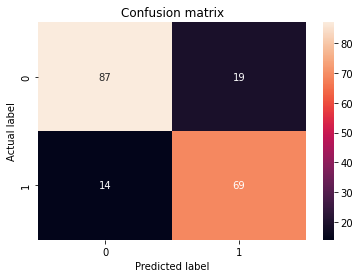
\includegraphics[width=4.5cm]{k-NN/k1_1.png}%
    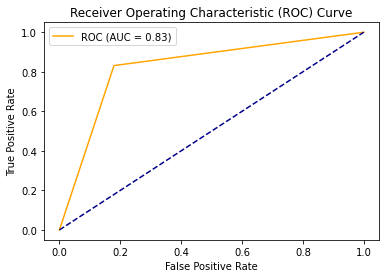
\includegraphics[width=4.5cm]{k-NN/k1_2.png}%
    \caption{Confusion Matrix & ROC Curve}%
    \label{fig:conf_KNN_1}%
\end{figure}

\subsubsection{Hyper-Parameter Selection Model}

The results for the Hyper-Parameter Selection Model are:

\begin{figure}[h!]
    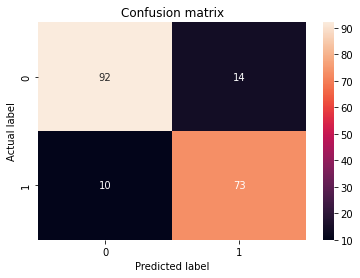
\includegraphics[width=4.5cm]{k-NN/k2_1.png}%
    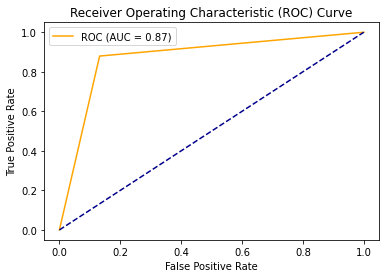
\includegraphics[width=4.5cm]{k-NN/k2_2.png}%
    \caption{2 Confusion Matrix & ROC Curve}%
    \label{fig:conf_KNN_2}%
\end{figure}

\subsubsection{K-Fold Cross-Validation Model}

The results for the K-Fold Cross-Validation Model are:

\begin{figure}[h!]
    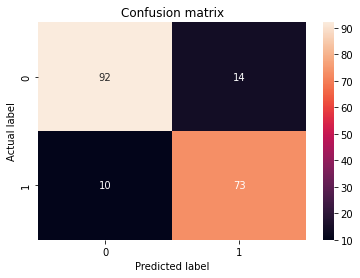
\includegraphics[width=4.5cm]{k-NN/k3_1.png}%
    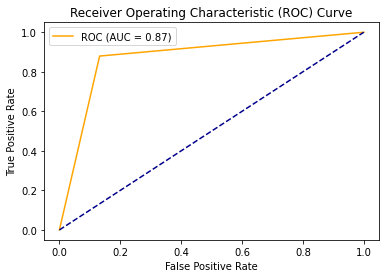
\includegraphics[width=4.5cm]{k-NN/k3_2.png}%
    \caption{Confusion Matrix & ROC Curve}%
    \label{fig:conf_KNN_3}%
\end{figure}

\begin{figure}[h!]
    \centering
    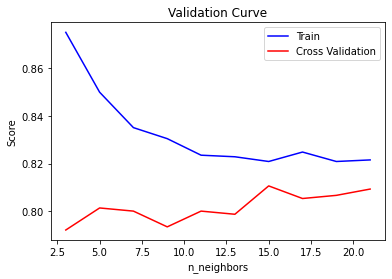
\includegraphics[width=4.5cm]{k-NN/k4.png}
    \caption{Validation Curve}
    \label{img:validationCurveKNN}
\end{figure}

\subsubsection{Conclusions}
As the graphics are very identical, a general conclusion will be made about the Confusion Matrix and ROC curve of all three implementations. As we can see, Fig. \ref{fig:conf_KNN_1}, \ref{fig:conf_KNN_2}, \ref{fig:conf_KNN_3} the Confusion Matrices are almost the same, so we see a bit of variation between the approaches, the ROC Curve is close to the top-left corner in the beginner, which is very good, how more the curve is closer to the top-left corner the better the performance, then the curve has a slope decrease to the end. About AUC (area under curve), how higher the value is (between 0 to 1) the better it is. As we can see in this article \cite{ROC_article}, values between 0.8 and 0.9 are considered excellent.

In Fig \ref{img:validationCurveKNN} , we can conclude that the ideal values for the parameter n\_neighbors are approximately 15 and 18.75. We also observed that from the value 15 of n\_neighbors, the accuracy of the training score and the Cross Validation score, remain more or less at the same values, with small descents and ascents, in the approximate values of 0.82 and 0.81 respectively.

\begin{table}[ht!]
    \centering
    \caption{Classification - All Model} 
    \begin{tabular}{||c| c c c||} 
    \hline
     & Accuracy & F1 Score & True Positive Rate \\ [0.5ex] 
     \hline\hline
     Base Model & 0.825 & 0.807 & 0.831 \\
     \hline
    Hyper-Parameter & 0.873 & 0.858 & 0.879 \\ 
    \hline
    K-Fold & 0.873 & 0.858 & 0.879 \\ 
    \hline
    \end{tabular}
    \label{tab:tab-final-knn}
\end{table}

So we can say (Table \ref{tab:tab-final-knn}) that with the K-NN model, the best approach is the Hyper-Parameter and the K-Fold, where the \textbf{Accuracy} is 0.873 and the \textbf{True Positive Rate} is 0.879.

%%%%%%%%%%%%%%%%%%%%%%%%%%%%%%%%%%%%%%%%%Decision Tree%%%%%%%%%%%%%%%%%%%%%%%%%%%%
\subsection{Decision Tree}


We run this model in three different ways, the base model, the hyper-parameter selection model, and the K-Fold cross-validation with the hyper-parameter selected. The following Table \ref{tab:tab6} shows the parameters chosen by the algorithm.

\begin{table}[h!]
    \centering
    \begin{tabular}{||c c c c c||} 
     \hline
     criterion & max\_depth & min\_samples\_leaf & min\_samples\_split & splitter \\[0.5ex] 
     \hline\hline
     entropy & 5 & 8 & 9 & random \\ 
    \hline
    \end{tabular}
    \caption{Best parameters in Decision Tree} 
    \label{tab:tab6}
\end{table}

\subsubsection{Base Model}
The results for the Base Model application are:

\begin{figure}[h!]
    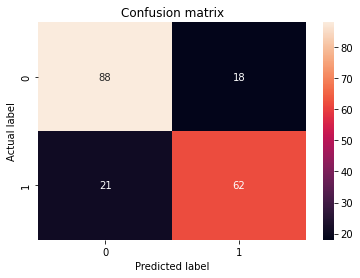
\includegraphics[width=4.5cm]{DT/dt1_1.png}%
    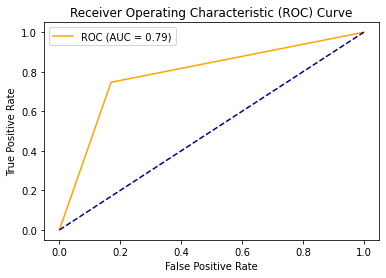
\includegraphics[width=4.5cm]{DT/dt1_2.png}%
    \caption{Confusion Matrix & ROC Curve}%
    \label{fig:conf_DT_1}%
\end{figure}

\subsubsection{Hyper-Parameter Selection Model}

The results for the Hyper-Parameter Selection Model are:

\begin{figure}[h!]
    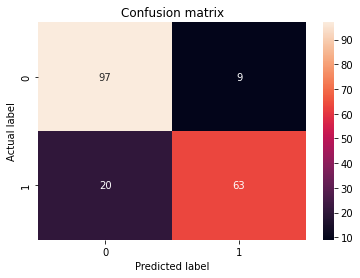
\includegraphics[width=4.5cm]{DT/dt2_1.png}%
    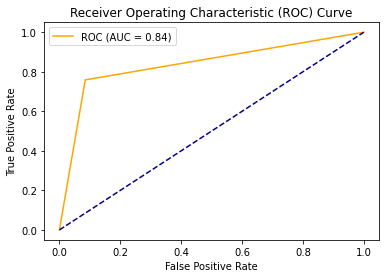
\includegraphics[width=4.5cm]{DT/dt2_2.png}%
    \caption{2 Confusion Matrix & ROC Curve}%
    \label{fig:conf_DT_2}%
\end{figure}

\subsubsection{K-Fold Cross-Validation Model}

The results for the K-Fold Cross-Validation Model are:

\begin{figure}[h!]
    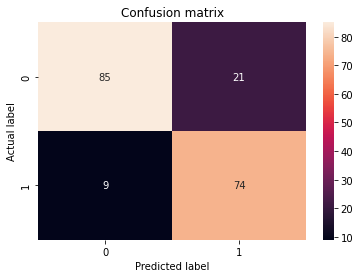
\includegraphics[width=4.5cm]{DT/dt3_1.png}%
    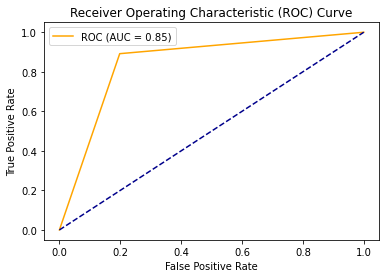
\includegraphics[width=4.5cm]{DT/dt3_2.png}%
    \caption{Confusion Matrix & ROC Curve}%
    \label{fig:conf_DT_3}%
\end{figure}

\begin{figure}[h!]
    \centering
    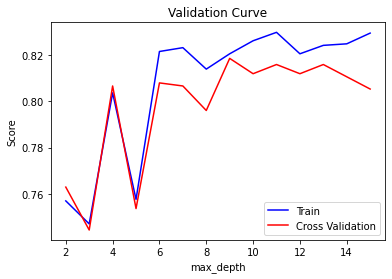
\includegraphics[width=4.5cm]{DT/dt4_1.png}
    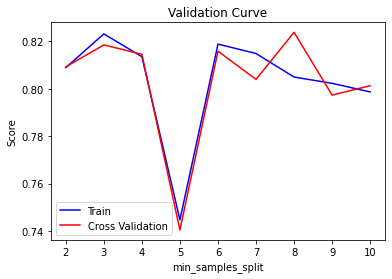
\includegraphics[width=4.5cm]{DT/dt4_2.png}
    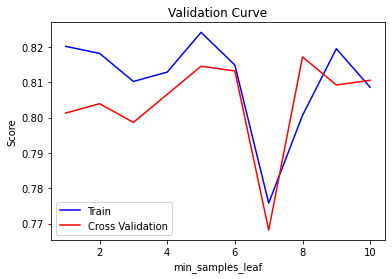
\includegraphics[width=4.5cm]{DT/dt4_3.png}
    \caption{Validation Curve}
    \label{img:validationCurveDT}
\end{figure}

\subsubsection{Conclusions}
As the graphics are very identical, a general conclusion will be made about the Confusion Matrix and ROC curve of all three implementations. As we can see, Fig. \ref{fig:conf_DT_1}, \ref{fig:conf_DT_2}, \ref{fig:conf_DT_3} the Confusion Matrices are almost the same, so we see a bit of variation between the approaches, the ROC Curve is close to the top-left corner in the beginner, which is very good, how more the curve is closer to the top-left corner the better the performance, then the curve has a slope decrease to the end. About AUC (area under curve), how higher the value is (between 0 to 1) the better it is. As we can see in this article \cite{ROC_article}, values between 0.8 and 0.9 are considered excellent.

In Fig \ref{img:validationCurveDT}, we see that both the max\_depth parameter and the min\_samples\_split parameter and min\_samples\_leaf can have any value, as they are practically all good, although there are better values (they are the intersection values of the train and the Cross Validation ), the difference is minimum.

\begin{table}[ht!]
    \centering
    \caption{Classification - All Model} 
    \begin{tabular}{||c| c c c||} 
    \hline
     & Accuracy & F1 Score & True Positive Rate \\ [0.5ex] 
     \hline\hline
     Base Model & 0.793 & 0.760 & 0.746 \\
     \hline
    Hyper-Parameter & 0.846 & 0.812 & 0.759 \\ 
    \hline
    K-Fold & 0.841 & 0.831 & 0.891 \\ 
    \hline
    \end{tabular}
    \label{tab:tab-final-tree}
\end{table}

So we can say (Table \ref{tab:tab-final-tree}) that with the Decision Tree model, the best approach is with K-Fold, where the \textbf{Accuracy} is 0.841 and the \textbf{True Positive Rate} is 0.891.

\subsection{Comparison between the models}

The comparison here \ref{tab:tab_comp_final} will be done with the best result from all models done in the previous section.

\begin{table}[ht!]
    \centering
    \caption{Classification - All Model} 
    \begin{tabular}{||c| c | c ||} 
    \hline
     ------ & Accuracy & True Positive Rate \\ [0.5ex] 
     \hline\hline
     Logistic Regression (HP/K-Fold) & 0.862 & 0.879 \\
     \hline
    Neural Network (Base Model) & 0.873 & 0.831 \\ 
    \hline
    SVC (HP/K-Fold) & 0.841 & 0.891 \\ 
    \hline
    K-NN (HP/K-Fold) & 0.841 & 0.891 \\ 
    \hline
    Decision Tree (K-Fold) & 0.831 & 0.891 \\ 
    \hline
    \end{tabular}
    \label{tab:tab_comp_final}
\end{table}

Three of the five have the best \textbf{True Positive Rate} (SVC (HP/K-Fold), K-NN (HP/K-Fold), Decision Tree (K-Fold)), which is 0.891, however, the SVC and K-NN approach have a little more of \textbf{Accuracy} (more 0.01), so we decided that the best model to our problem will be one of the (SVC (HP/K-Fold) or K-NN (HP/K-Fold) approach.

\section{Novelty and contributions}

We found a published article A Machine Learning Predictive Model to Classify Severity of Breast Cancer Based on Mammographic Mass Dataset \cite{nov} that has the following results:

\begin{figure}[h!]
    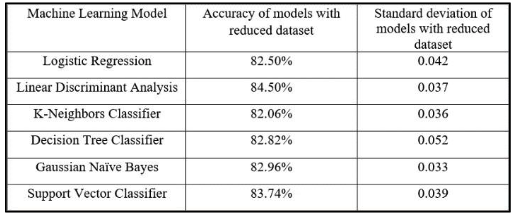
\includegraphics[width=8cm]{novely_results.png}%
    \caption{Published Reference Results}%
    \label{fig:novely_result}%
\end{figure}

Comparing our solution with theirs at accuracy levels (they don't have information about \textbf{True Positive Rate}), we have some models with more accuracy (Logistic Regression (HP/K-Fold) - 0.862 and Neural Network (Base Model) - 0.873) that the best of their (Linear Discriminant Analysis - 0.845).

We can say that we propose a better solution, with better performance of the Machine Learning models.

\section{Conclusion}

Doing this project was very relevant since we not only successfully applied the machine learning algorithms learned in class, but we also self-learned new technics of machine learning using the internet. 
As we were developing our work, there were some periods where we found some difficulties, especially when we were dealing with data preprocessing since we had trouble deciding which features should be discarded. If we were to develop this work even further we would like to improve our data preprocessing or have more features in order to have better results.
 In the end, we are very content with the work we presented, since it made us increase our knowledge.


\printbibliography

\end{document}
